\chapter{Identification \& Authentication}

\section{Einführung}

``Identification \& Authentication'' (I\&A) fasst folgende zwei Schritte zusammen:

\begin{enumerate}
	\item Feststellen der Identität eines Subjektes sowie Verbindung zu einer im System abgelegten ID herstellen (Identification)
	\item Mittels einem Authenticator\footnote{Als Authenticator gilt z.B. ein Passwort, Hardwaretoken, Streichliste usw.} prüfen, ob Subjekt wirklich für die ermittelte ID berechtigt ist (Authentication)
\end{enumerate}

Für dieses grundlegende Schema gibt es zwei verschiedene Varianten:

\begin{enumerate}
	\item Ein Subjekt wird mit einer eindeutigen Identität in Verbindung gebracht (Individual I\&A)
	\item Ein Subjekt wird lediglich auf die Zugehörigkeit zu einer Gruppe geprüft (Group I\&A)\\
	Beispiel: Wache prüft jede Person an der Pforto, ob er einen Mitarbeiterbadge bei sich trägt.
\end{enumerate}

Um I\&A einsetzen zu können ist eine Reihe weiterer (aktiver und passiver) Komponenten nötig:
\begin{itemize}
	\item \emph{Subjektregistrierung}: Ein Subjekt muss initial registriert werden, damit es später wieder identifizert und authentifiziert werden kann
	\item \emph{Sessionmanagement}: Schlagwort Single-Sign-On
	\item \emph{Gesicherte Systemkomponenten, ``Using function''}: Komponenten, welche I\&A aufrufen und dessen Output verwenden (z.B. Patterns aus dem Kapitel \ref{sec:accesscontrolmodels})
\end{itemize}

\begin{figure}[H]
	\centering
	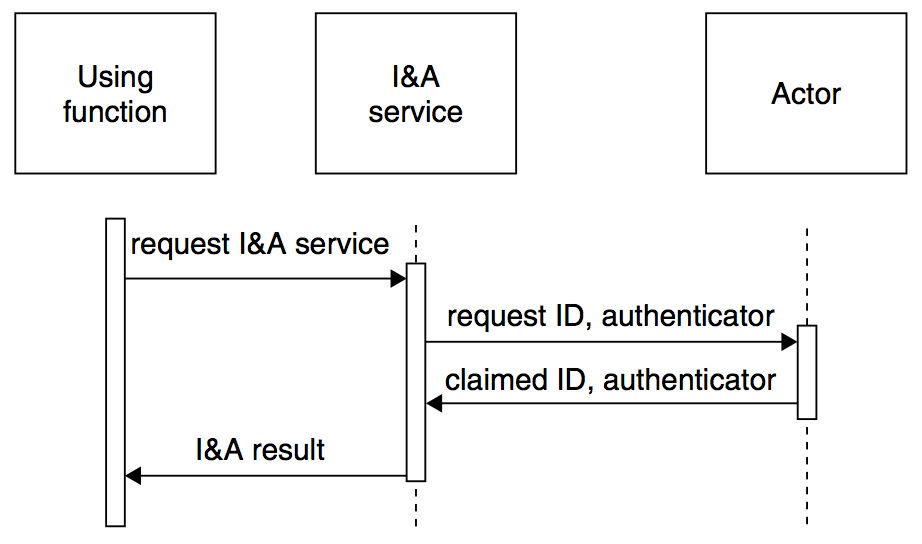
\includegraphics[width=8cm]{content/identification-and-authentication/using-functions.png}
	\caption{Generischer Ansatz von I\&A ``Using functions'' \cite{SecPatterns06}}
\end{figure}

\subsection*{Mögliche Prüfungsfragen}
\begin{itemize}
	\item \emph{Was ist ein Authenticator?}\\
	Nachdem ein Subjekt mit einer im System abgelegten Identität in verbindung gebracht wurde, wird der Authenticator verwendet, um sicherzustellen, dass das Subjekt auch wirklich das Subjekt ist, für welches es sicht ausgibt.\\
	Beispiel: Nach Eingabe des Benutzernamens wird das Passwort als Authenticator verwendet.

	\item \emph{Welche grundlegenden Typen von I\&A unterscheidet man?}\\
	Individual und Group Identification \& Authentication
\end{itemize}

\section{I\&A Requirements}

Muss ein I\&A Service etabliert werden, hilft das I\&A Requirements Pattern mit seinen generischen Requirementsvorlagen bei der Analyse eines bestehenden oder zu konzipierenden Systems.

Dabei werden nicht nur sicherheitsrelevante Faktoren berücksichtigt. Aspekte wie Kosteneffektivität oder Benutzerzufriedenheit und -akzeptanz fliessen ebenso in die Analyse mitein.

\subsection*{Kontext}
Eine Organisation oder ein Projekt konzipiert die Verwendung von I\&A. Das Pattern unterstützt die Analyse jeglicher Situationen, in welchen sowohl Identification als auch Authorization notwendig ist.

\subsection*{Problem}


\subsection*{Lösung}


\subsection*{Erweiterungen}

\subsection*{Vorteile}
\begin{itemize}
	\item 
\end{itemize}

\subsection*{Nachteile}
\begin{itemize}
	\item 
\end{itemize}

\subsection*{Beispielanwendungen}
\begin{itemize}
	\item 
\end{itemize}

\subsection*{Mögliche Prüfungsfragen}
\begin{itemize}
	\item \emph{adasd?}\\
	dasd
\end{itemize}